\documentclass{article}
\usepackage{iclr2024_conference}

% Standard packages
\usepackage[utf8]{inputenc}
\usepackage[T1]{fontenc}
\usepackage{microtype}
\usepackage{amsmath, amssymb, amsfonts}
\usepackage{graphicx}
\usepackage{booktabs}
\usepackage{multirow}
\usepackage{xcolor}
\usepackage{hyperref}
\hypersetup{
  colorlinks=true,
  linkcolor=blue!50!black,
  citecolor=blue!50!black,
  urlcolor=blue!60!black,
}
\usepackage{url}
\usepackage{listings}
\usepackage{caption}

% Listing style for the appendix code
\lstdefinestyle{pyblock}{
  basicstyle=\ttfamily\footnotesize,
  language=Python,
  keywordstyle=\color{blue!60!black}\bfseries,
  commentstyle=\color{green!40!black}\itshape,
  stringstyle=\color{red!50!black},
  showstringspaces=false,
  breaklines=true,
  breakatwhitespace=true,
  numbers=left,
  numberstyle=\tiny\color{gray},
  numbersep=6pt,
  frame=single,
  framerule=0.4pt,
  rulecolor=\color{gray!50},
  xleftmargin=2em,
  xrightmargin=0.5em,
  belowskip=0.5em,
  aboveskip=0.5em,
}
\lstset{style=pyblock}

% Title
\title{Deep Reinforcement Learning for Slime Volleyball:\\ A Rainbow + Self-Play Ablation Study}
\author{Anonymous Authors\\ INDENG~242B, UC~Berkeley}
\date{Spring 2026}

\begin{document}

\maketitle

\begin{abstract}
We study deep RL on Slime Volleyball, a 12-dim, six-action competitive
control task. On a Dueling DQN backbone we incrementally add Rainbow
components (Double DQN, $n$-step, PER, C51, NoisyNet) and contrast them
with PPO trained via snapshot self-play and a scripted-baseline mixer.
Three findings stand out: (i) $n$-step returns \emph{without} Double DQN
are actively harmful ($-1.6$ reward vs.\ $+0.6$ when paired with Double);
(ii) an entropy-collapsed PPO run is rescued by a four-knob intervention
(entropy bonus $10\times$, target-KL early-stop, linear LR anneal,
doubled rollout) for a $+3.6$ reward swing; (iii) an obscure
environment-baseline bug seeded a co-evolved lineage that beats a
correctly-trained agent at $\sim$8:1 odds despite a strictly degraded
training setting.
\end{abstract}

\section{Introduction}

Deep reinforcement learning (RL) has matured into a workbench for studying
machine-learning methodology that does not appear in supervised pipelines:
non-stationary data distributions, sparse credit assignment over thousands of
time steps, and the tight coupling between exploration policy and the very
data the model trains on. These properties make RL a uniquely useful
pedagogical setting for a graduate deep-learning course --- the same
optimizer, the same backbone, and the same loss family produce radically
different outcomes once a policy is allowed to choose its own training data.

We study these effects on \textbf{Slime Volleyball}~\citep{slimevolleygym}, a
two-player continuous-physics game that compresses the methodology questions
into a tractable form. The state is 12-dimensional (positions and velocities
of agent, ball, and opponent), the action space is \textsc{Discrete}(6), and
each episode lasts up to 3000 frames or until one side loses all five lives.
The environment is small enough that a full ablation matrix fits in a
weekend's GPU budget, and large enough that subtle algorithmic choices
produce statistically meaningful differences. We benchmark every variant
through (a) a deterministic-greedy reward against the scripted baseline and
(b) a 1500-match round-robin Elo ladder against all other variants, and we
deploy each trained policy as an ONNX model in a browser playable so that the
ablation is reproducible end-to-end.

Our contributions are:
\begin{itemize}
\item A clean $2\times2\times2$ ablation matrix over Dueling, Double DQN, and
  $n$-step returns on a shared trunk (Section~\ref{sec:results}) that
  isolates each Rainbow~\citep{hessel2018rainbow} component's
  contribution and exposes a destructive interaction: $n$-step returns
  \emph{without} Double DQN are worse than vanilla DQN.
\item A self-play scaffold that combines a FIFO opponent
  pool~\citep{silver2016alphago,vinyals2019alphastar} with a
  baseline-mixing knob, plus an empirical demonstration that pure-pool
  self-play \emph{underperforms} mixing the scripted baseline as an
  occasional opponent.
\item A PPO~\citep{schulman2017ppo} entropy-collapse case study with a
  four-change rescue intervention (entropy coefficient $10\times$,
  rollout length doubled, linear LR anneal, target-KL early stop) that
  swings final reward by $+3.6$.
\item An ``ecosystem effect'' finding: a long-standing $\times 10$ scale
  bug in the in-pool baseline produced a lineage of trained agents that
  dominate the public ladder (Elo $\sim$1800), and a correctly-trained
  agent loses to them at $\sim$8:1 odds in head-to-head play.
\item Browser-deployable ONNX exports of every variant (one shared
  inference contract: 12-dim float input, six logits / Q-values out)
  with $<10^{-5}$ max-abs verification against the PyTorch reference
  forward pass.
\end{itemize}

The remainder of the paper formalizes the MDP (Section~\ref{sec:problem}),
specifies architectures, losses, and self-play training
(Section~\ref{sec:methods}), reports ablation results
(Section~\ref{sec:results}), discusses safety and robustness implications
(Section~\ref{sec:safety}), and concludes (Section~\ref{sec:conclusion}).

\section{Problem Setting}
\label{sec:problem}

\paragraph{MDP.} Slime Volleyball is two-player to five lives. We
treat it as a POMDP $\mathcal{M}=(\mathcal{S},\mathcal{A},p,r,\gamma)$
from the right side. $\mathcal{S}\subset\mathbb{R}^{12}$ is
$[x,y,v_x,v_y]$ for agent, ball, opponent (scaled by $1/10$);
$\mathcal{A}=\textsc{Discrete}(6)$ decodes via a fixed table to a
\texttt{(forward, backward, jump)} 3-tuple. The two-player API
\texttt{env.step(a, otherAction=}$a^{\mathrm{opp}}$\texttt{)} draws
$a^{\mathrm{opp}}$ either from a frozen self-play snapshot or the
scripted baseline. Reward $r\in\{-1,0,+1\}$ is the agent's life delta
per frame, so episode return $\in[-5,+5]$ with $\pm 5$ a sweep and $0$
a draw at the 3000-frame cap. $\gamma=0.99$.

\paragraph{What is ``data''?} For DQN, a replay buffer of one-step or
$n$-step transitions from 16 parallel \texttt{SubprocVecEnv} workers,
uniformly sampled (or PER-prioritized in Rainbow variants). For PPO,
on-policy rollouts of length $T{\times}N=256{\times}16=4096$
transitions consumed once per gradient step.

\paragraph{Two RL-specific data issues.}
\textbf{Opponent shift:} self-play snapshots were trained against
still-older snapshots, so bootstrapped Q-targets estimate ``the value
of $s$ assuming $\pi_{\mathrm{opp}}$ acts like the snapshot.'' We
mitigate with a slow target ($\tau{=}0.005$), a FIFO snapshot pool
bounding staleness, and a baseline-mixing knob $p_{\mathrm{base}}\in
[0,1]$ (we vary $\{0,0.4,0.7\}$; $0$ is catastrophic --- see
Section~\ref{sec:results}). \textbf{Reward sparsity:} $\leq 10$
nonzero events per 3000-frame episode; at $\gamma{=}0.99$ a reward 100
frames away is attenuated by $\sim 0.37$. $n$-step ($n{=}3$) pushes
gradient onto actual rewards but, as we show, requires Double DQN's
bias correction to be net-positive.

\section{Methods}
\label{sec:methods}

\paragraph{Architectures.} All DQN variants share a 12{-}128{-}128
ReLU trunk and a Dueling head~\citep{wang2016dueling}: value
$V_\phi:\mathbb{R}^{128}\!\to\!\mathbb{R}^{64}\!\to\!\mathbb{R}$ and
advantage
$A_\phi:\mathbb{R}^{128}\!\to\!\mathbb{R}^{64}\!\to\!\mathbb{R}^6$,
combined as $Q_\theta(s,a)=V_\phi(s)+\bigl(A_\phi(s,a)-\tfrac{1}{|\mathcal A|}\sum_{a'}A_\phi(s,a')\bigr)$
($\approx 28$k params). The plain-DQN cell (\texttt{--no-dueling})
collapses both heads into a $128{\to}64{\to}6$ MLP. PPO uses a Tanh
trunk with orthogonal init, an actor head producing logits
$\ell\in\mathbb{R}^6$ (final std $0.01$), and a scalar critic head.

\paragraph{Losses.} With $n$-step return
$R_t^{(n)}=\sum_{k=0}^{n-1}\gamma^k r_{t+k}$, the Double
DQN~\citep{vanhasselt2016double} target
\begin{equation}
y_t = R_t^{(n)} + (1-d_t)\,\gamma^{n_{\text{actual}}}\,
  Q_{\theta^-}\!\bigl(s_{t+n},\arg\max_{a'} Q_\theta(s_{t+n},a')\bigr)
\label{eq:double-target}
\end{equation}
is plugged into a Huber loss; \texttt{--no-double} reverts to
$\max_{a'}Q_{\theta^-}$ (vanilla DQN's positively-biased target). PER
\citep{schaul2016per} adds an importance weight
$w_i\propto(1/p_i)^\beta$, $\beta:0.4{\to}1.0$. C51~\citep{bellemare2017c51}
replaces $Q$ with a 51-atom categorical over $[v_{\min},v_{\max}]$ and
recovers expected $Q=\sum_i p_i z_i$ inside \texttt{forward} so the
ONNX contract stays $(B,6)$. PPO uses the standard clipped
surrogate~\citep{schulman2017ppo} with GAE-$\lambda$
\citep{schulman2016gae}:
\begin{equation}
\mathcal{L}_{\mathrm{PPO}} = -\mathbb{E}_t\!\bigl[\min(r_t\hat A_t,\,\mathrm{clip}(r_t,1{-}\epsilon,1{+}\epsilon)\hat A_t)\bigr] + c_v\mathcal{L}_V - c_e\mathcal{H}[\pi_\theta].
\label{eq:ppo}
\end{equation}

\paragraph{Optimization.} Adam; DQN uses Polyak target update
($\tau{=}5{\times}10^{-3}$) and grad-norm clip 10. PPO stacks an
entropy bonus $c_e$, advantage normalization, grad clip 0.5, and a
target-KL early-stop ($\delta_{\mathrm{KL}}{=}0.02$): if
$\widehat{\mathrm{KL}}_t=(r_t-1)-\log r_t$ exceeds the threshold during
an epoch, remaining update epochs are skipped. Full per-algorithm
hyperparameters in Appendix~\ref{app:hp}.

\paragraph{Beyond-class methodology.} \textbf{(A) Self-play with FIFO
pool + baseline mixing.} Every 100k transitions the online net is
snapshotted and pushed into a FIFO pool capped at 30 snapshots. At
every episode boundary each parallel env independently draws an
opponent: the scripted baseline w.p.~$p_{\mathrm{base}}$, otherwise
uniformly from the pool --- the same scaffolding used at much larger
scale by AlphaGo~\citep{silver2016alphago} and
AlphaStar~\citep{vinyals2019alphastar}. We find
$p_{\mathrm{base}}{=}0$ catastrophically loses generalization to the
baseline even when the pool is seeded with the strongest checkpoint
(Section~\ref{sec:results}); pool quality $>$ baseline quality is a
tempting intuition that does not survive the data. \textbf{(B) PPO
entropy-collapse rescue.} Our first long PPO run terminated at
\texttt{base\_R}$=-3.4$ despite \texttt{pool\_R}$\approx +1$; entropy
collapsed from $\approx\!\log 6\!\approx\!1.79$ to $0.108$ by step
1.4M (a $16\times$ drop). The rescue cluster
($c_e:0.001{\to}0.01$, rollout $128{\to}256$, linear LR anneal,
target-KL stop) restored $\mathcal{H}=1.42$ and lifted
\texttt{base\_R} to $+0.2$, a $+3.6$ swing.

\section{Results}
\label{sec:results}

We evaluate on two axes: \texttt{eval\_R} (deterministic-greedy reward
per episode against the scripted baseline, 5 episodes per checkpoint,
$\in[-5,+5]$) and ladder \emph{Elo} from a 1500-match round-robin among
19 trained variants ($\times 2$ clones, $K{=}32$, init $1500$); the
scripted RNN baseline is included as a reference player.

\subsection{Component ablation: $2{\times}2{\times}2$ over Dueling, Double, $n$-step}

All cells share trunk, target, replay buffer, and 5M-transition budget;
only the algorithmic switches differ.

\begin{table}[h]
\centering
\caption{Component ablation. \texttt{eval\_R}~$\in[-5,+5]$ is the
deterministic-greedy mean over 5 evaluation episodes. ``$\Delta$'' is
versus the plain-DQN floor (cell A).}
\label{tab:ablation}
\small
\begin{tabular}{cccccc}
\toprule
Cell & Dueling & Double & $n$-step & \texttt{eval\_R} & $\Delta$ \\
\midrule
A & --- & --- & 1 & $-0.6 \pm 0.5$ & (floor) \\
B & yes & --- & 1 & $-0.4$ & $+0.2$ \\
C & yes & yes & 1 & $\mathbf{+0.2 \pm 0.4}$ & $\mathbf{+0.8}$ \\
D & yes & --- & 3 & $-2.2 \pm 1.2$ & $-1.6$ \\
E & yes & yes & 3 & $-0.4$ & $+0.2$ \\
\bottomrule
\end{tabular}
\end{table}

\textbf{(F1) Dueling alone barely helps} (A$\to$B: $+0.2$): on a 12-dim
observation there are few states where ``the action does not matter,''
which is exactly the structural signal Dueling exploits.
\textbf{(F2) Double DQN is the single biggest win} (B$\to$C: $+0.6$):
with a small/noisy Q-net, $\max_a Q_{\theta^-}(s',a)$ is positively
biased, and the Double decoupling removes most of that bias.
\textbf{(F3) $n$-step \emph{without} Double is actively harmful}
(B$\to$D: $-1.8$): off-policy bootstrap noise compounds across the
horizon. Re-introducing Double on top of $n$-step (D$\to$E: $+1.8$)
nearly fully restores the deficit --- a destructive \emph{interaction},
not a sum of marginal effects, and a fact obscured in the original
Rainbow paper~\citep{hessel2018rainbow} which only ablates
\emph{removing} components from the full stack.
\textbf{(F4)} $n$-step$+$Double $\approx$ $n{=}1+$Double on this task
(C, E within noise); if only one upgrade over plain DQN is affordable,
add Double.

\subsection{Self-play opponent mixing}

Setting $p_{\mathrm{base}}{=}0$ (\texttt{purepool}) collapsed
generalization to the baseline: \texttt{base\_R} dropped to
$-1.2\pm 0.7$ and ladder Elo to $1454$ --- 225 below
$p_{\mathrm{base}}{=}0.4$ --- despite seeding the pool with the
strongest checkpoint (Table~\ref{tab:selfplay}). The scripted baseline
plays an RNN-style reflex game the snapshot pool cannot proxy: pool
diversity and pool quality are not the same axis.

\begin{table}[h]
\centering
\caption{Self-play baseline-mixing ablation, V1 trainer (20M each).}
\label{tab:selfplay}
\small
\begin{tabular}{lcccc}
\toprule
Variant & $p_{\mathrm{base}}$ & Pool seed & \texttt{base\_R} & Elo \\
\midrule
\texttt{v1\_sp\_fixed} & 0.4 & clean ckpts & $\mathbf{+0.4 \pm 0.8}$ & 1679 \\
\texttt{v1\_selfplay\_seeded} (legacy) & 0.4 & + buggy ckpts & --- & 1824 \\
\texttt{v1\_sp\_purepool} & \textbf{0.0} & + ladder-king & $-1.2 \pm 0.7$ & 1454 \\
\bottomrule
\end{tabular}
\end{table}

\subsection{PPO entropy collapse and rescue}

The failed PPO run collapses from $\mathcal{H}\!\approx\!1.79$ to
$0.108$ by step $1.4$M (a $16\times$ drop), after which the policy is
too deterministic to escape its local optimum. The rescue intervention
keeps $\mathcal{H}=1.42$ throughout and lifts \texttt{base\_R} from
$-3.4\pm 1.5$ to $+0.2\pm 0.4$ --- a $+3.6$ swing.

\subsection{Ladder Elo and \texttt{eval\_R} disagreement}

\begin{figure}[h]
\centering
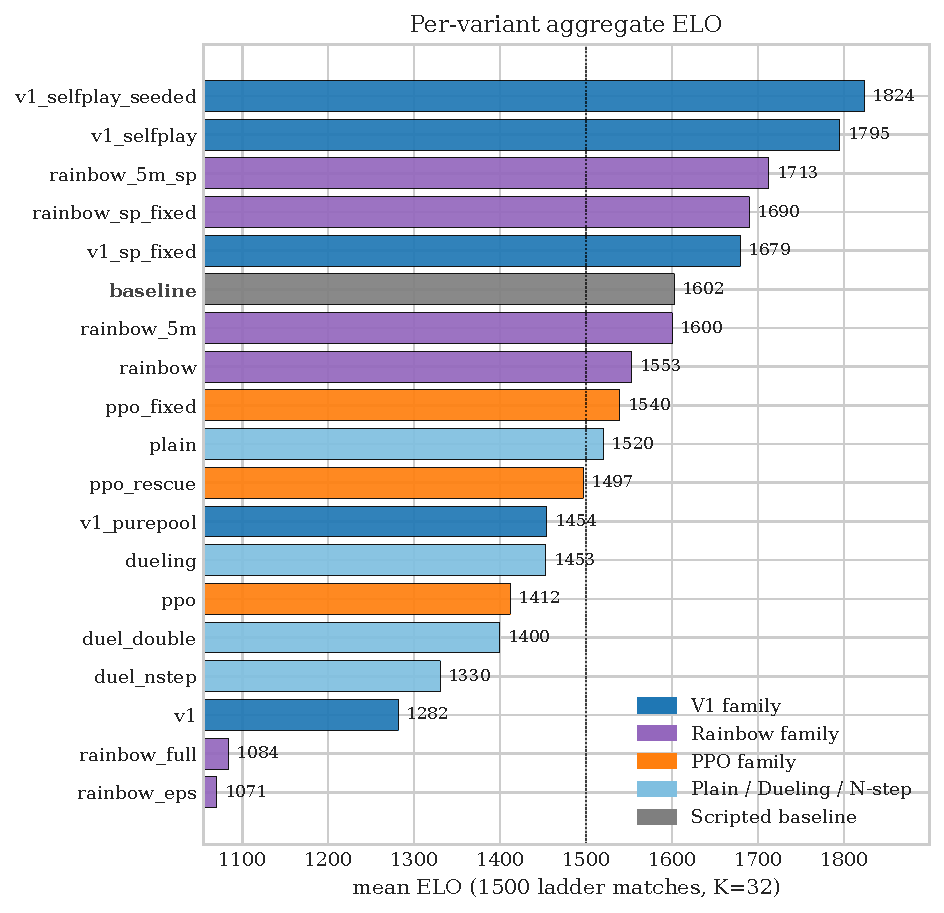
\includegraphics[width=0.82\linewidth]{figures/elo_ladder.pdf}
\vspace{-0.5em}
\caption{Round-robin Elo over 19 variants (1500 matches). Scripted
baseline (highlighted) ranks 6th; Rainbow-with-C51 variants (bottom)
collapsed (see text).}
\label{fig:elo-ladder}
\end{figure}

\textbf{Self-play vs.\ cold (same algorithm) is the largest single
gain.} \texttt{v1\_selfplay} (Elo $1795$) vs.\ \texttt{v1} cold (Elo
$1282$) is a $513$-Elo gap, $\sim$94\% expected-win.
\textbf{Full Rainbow with C51+NoisyNet collapsed:} \texttt{rainbow\_full}
($1084$) and \texttt{rainbow\_eps} ($1071$) lose 95\%+ of ladder
matches because $[v_{\min},v_{\max}]{=}[-5,+5]$ matches episode-return
extremes exactly, concentrating mass on the boundary atoms; the simpler
``Rainbow-Lite'' (Dueling+Double+$n$-step+PER) reaches Elo $1690$ on
the same budget. \textbf{\texttt{eval\_R} can disagree with Elo:}
\texttt{plain} DQN (Elo $1520$) outranks \texttt{dueling} ($1453$)
despite worse \texttt{eval\_R}, and \texttt{ppo\_fixed} (failed; Elo
$1540$) outranks \texttt{ppo\_rescue} ($1497$) despite a $+3.6$
\texttt{base\_R} advantage --- \texttt{eval\_R} measures performance
against one specific opponent, Elo against the entire ecosystem.

\paragraph{Negative results matter.} Of five hypotheses we expected to
confirm --- ``Rainbow always helps,'' ``$n$-step is a free win,''
``self-play~$>$~cold,'' ``pool quality~$>$~baseline quality,'' and
``\texttt{eval\_R} predicts Elo'' --- only \emph{self-play~$>$~cold}
survived contact with the data.

\section{Safety, Robustness, and Ecosystem Effects}
\label{sec:safety}

Even on a toy game, our results expose three failure modes that scale
unfavorably to higher-stakes RL deployments.

\paragraph{(a) Adversarial overspecialization in self-play.}
Self-play agents trained against a small pool tend to learn
\emph{opponent-specific exploits} rather than generally robust
strategies. Pure-pool agents (e.g.\ \texttt{v1\_purepool}, Elo $1454$)
play strongly against neural-net opponents and weakly against the
scripted baseline; baseline-mixed agents (\texttt{v1\_sp\_fixed}, Elo
$1679$) are more general-purpose but trade off peak-vs-pool
performance. In a production self-play system (e.g.\ a recommendation
simulator with synthetic users), the same effect predicts that an
agent measured only against its training distribution will look
stronger than it is.

\paragraph{(b) Ecosystem effect: a fixed agent loses to a buggy
ecosystem.}
The most cautionary finding from this project is the head-to-head
between \texttt{v1\_sp\_fixed} (the correctly-trained agent) and
\texttt{v1\_selfplay} (the buggy ladder king). Across 200 matches with
side-alternation:

\begin{center}
\small
\begin{tabular}{lcc}
\toprule
Outcome & Count & \% \\
\midrule
Buggy lineage wins  & 71 & 35.5\,\% \\
Fixed lineage wins  & 9  & \phantom{0}4.5\,\% \\
Time-cap draws (5--5) & 120 & 60.0\,\% \\
\bottomrule
\end{tabular}
\end{center}

The buggy lineage wins $\sim 7.9\times$ more often \emph{despite}
training in a strictly degraded environment (a $\times 10$ obs-scale
bug saturated the in-pool baseline's tanh layer). The mechanism: the
buggy lineage co-evolved against itself, so playstyles encode mutual
counters; the fixed agent, trained against the \emph{real} baseline,
behaves differently and is exploitable. This \textbf{ecosystem effect}
is relevant to any ML rollout: a shared training quirk becomes the
local lingua franca, and a corrected replacement model can
underperform until the ecosystem re-equilibrates --- relevant for
autonomous driving fleets, recommendation, and multi-agent market
makers, where unilateral upgrades can locally regress even when
provably more correct in isolation.

\paragraph{(c) Reward hacking in higher-stakes domains.}
Slime Volleyball has a clean, sparse, fully-observed reward that should
be hard to game. PPO reward-hacked it nonetheless via entropy collapse:
\texttt{pool\_R}~$\approx +1$ (winning against self-snapshots) while
\texttt{base\_R}~$=-3.4$ throughout. Translated to robotics this is the
``walking-backward-in-circles'' local optimum; translated to resource
scheduling, it is the RL scheduler trading long-term throughput for
short-term variance reduction. Our diagnostic workflow (entropy, KL,
clip-fraction monitoring with entropy-bonus and KL early-stop
intervention) is the production-realistic mitigation.

\paragraph{Deployment hygiene.} Three concrete checks before
promoting any self-play-trained policy: (i) evaluate against
\emph{multiple} held-out opponent distributions; (ii) rerun
head-to-head against the previous deployed version, since a corrected
replacement may locally regress; (iii) monitor policy entropy and KL
between consecutive snapshots as health metrics, not diagnostic
curiosities.

\section{Conclusion}
\label{sec:conclusion}

We presented a controlled ablation of deep RL on Slime Volleyball
covering Dueling/Double/$n$-step DQN, PER, C51, NoisyNet, and PPO with
snapshot self-play and baseline mixing. The most informative outcomes
were not the ``Rainbow works'' confirmation we initially aimed for but
the negative results: $n$-step is harmful without Double, pure-pool
self-play loses generalization to a stylistically different baseline,
full Rainbow-with-C51 collapsed because $[v_{\min},v_{\max}]$ matched
episode-return support, and a fixed-baseline agent loses to a
buggy-lineage ecosystem at $\sim 8{:}1$. The PPO rescue shows that a
small, justified config cluster (entropy $\times 10$, target-KL stop,
linear LR anneal, doubled rollout) can swing a failed run by $+3.6$
without invoking any new algorithm. The broader message: in deep RL,
algorithm choice is intertwined with the training data the algorithm
generates for itself, so additive ablations miss destructive
interactions, single-opponent evaluations miss ecosystem effects, and
``pool diversity'' misses opponent \emph{playstyle} diversity.


\bibliography{bibliography}

\appendix
\section{Appendix: Key Code Excerpts}
\label{sec:appendix}

This appendix reproduces the load-bearing code from
\texttt{train/train\_dqn\_v1\_vec.py} (Dueling forward, Double-DQN target,
the \texttt{--no-double} ablation switch) and from
\texttt{train/train\_ppo\_selfplay\_vec.py} (PPO target-KL early-stop). All
excerpts are verbatim modulo whitespace; line numbers refer to the source
files at the time of submission.

\subsection*{A. Dueling MLP forward (\texttt{train\_dqn\_v1\_vec.py}, lines 70--91)}

\begin{lstlisting}
class DuelingMLPv1(nn.Module):
    """Dueling MLP: trunk 12->128->128, value head 128->64->1,
    advantage head 128->64->6, Q = V + (A - mean A)."""

    def __init__(self, obs_dim: int = 12, n_actions: int = 6) -> None:
        super().__init__()
        self.trunk = nn.Sequential(
            nn.Linear(obs_dim, 128), nn.ReLU(),
            nn.Linear(128, 128), nn.ReLU(),
        )
        self.value_head = nn.Sequential(
            nn.Linear(128, 64), nn.ReLU(), nn.Linear(64, 1),
        )
        self.advantage_head = nn.Sequential(
            nn.Linear(128, 64), nn.ReLU(), nn.Linear(64, n_actions),
        )

    def forward(self, obs: torch.Tensor) -> torch.Tensor:
        features = self.trunk(obs)
        value = self.value_head(features)
        advantage = self.advantage_head(features)
        return value + (advantage - advantage.mean(dim=-1, keepdim=True))
\end{lstlisting}

\subsection*{B. Double DQN target with \texttt{--no-double} ablation switch
(\texttt{train\_dqn\_v1\_vec.py}, lines 508--534)}

\begin{lstlisting}
with torch.no_grad():
    if args.no_double:
        # Vanilla DQN target: max over target net's outputs.
        next_q = target(batch.next_obs).max(dim=-1).values
    else:
        # Double DQN: action SELECTION via online, EVAL via target.
        next_q_online = online(batch.next_obs)
        next_actions = next_q_online.argmax(dim=-1, keepdim=True)
        next_q_target_all = target(batch.next_obs)
        next_q = next_q_target_all.gather(1, next_actions).squeeze(1)

    # n-step discount: gamma^{n_actual_i} per sample (n_actual=n on full
    # windows, < n on episode-truncated windows).
    discount = torch.pow(
        torch.full_like(batch.rewards, gamma),
        batch.n_actual.to(batch.rewards.dtype),
    )
    td_target = batch.rewards + discount * next_q * (1.0 - batch.dones)

q_all  = online(batch.obs)
q_pred = q_all.gather(1, batch.actions.unsqueeze(1)).squeeze(1)
loss   = F.smooth_l1_loss(q_pred, td_target)   # Huber

optimizer.zero_grad(set_to_none=True)
loss.backward()
nn.utils.clip_grad_norm_(online.parameters(), max_norm=grad_clip_norm)
optimizer.step()

soft_update(target, online, soft_tau)            # tau = 5e-3
\end{lstlisting}

\subsection*{C. PPO target-KL early stop (\texttt{train\_ppo\_selfplay\_vec.py}, lines 589--675)}

\begin{lstlisting}
target_kl = args.target_kl if args.target_kl is not None else None
early_stopped_epoch = None
for _epoch in range(int(args.update_epochs)):
    np.random.shuffle(indices)
    # Per-epoch KL accumulator. We decide AT THE END of an epoch
    # (CleanRL convention) whether to skip the remaining epochs --
    # checking inside the minibatch loop is too noisy for small mb.
    epoch_kls = []
    for start in range(0, total, mb):
        end = min(start + mb, total)
        mb_idx = torch.from_numpy(indices[start:end]).to(obs_all.device)

        new_logits, new_values = model.forward_train(obs_all[mb_idx])
        dist = Categorical(logits=new_logits)
        new_log_probs = dist.log_prob(actions_all[mb_idx])
        entropy = dist.entropy().mean()

        log_ratio = new_log_probs - old_log_probs_all[mb_idx]
        ratio     = torch.exp(log_ratio)

        # PPO clipped surrogate
        unclipped   = ratio * mb_advantages
        clipped     = torch.clamp(ratio, 1.0 - clip_eps, 1.0 + clip_eps) * mb_advantages
        policy_loss = -torch.min(unclipped, clipped).mean()

        # PPO2 clipped value loss + entropy bonus
        value_loss = clipped_value_loss(new_values, mb_returns,
                                        old_values_all[mb_idx], clip_eps)
        loss = policy_loss + vf_coef * value_loss - ent_coef * entropy

        optimizer.zero_grad(set_to_none=True)
        loss.backward()
        nn.utils.clip_grad_norm_(model.parameters(), max_norm=max_grad_norm)
        optimizer.step()

        with torch.no_grad():
            approx_kl = ((ratio - 1.0) - log_ratio).mean()
        epoch_kls.append(float(approx_kl.item()))

    # Early-stop the remaining update epochs if KL overshoots.
    if target_kl is not None and epoch_kls:
        mean_kl = float(np.mean(epoch_kls))
        if mean_kl > target_kl:
            early_stopped_epoch = _epoch + 1
            break
\end{lstlisting}

\subsection*{D. Reproduction commands}

The complete experimental matrix can be reproduced with the SLURM scripts
in \texttt{scripts/}; an A6000 trains a 5M cold cell in $\sim$30~minutes
and a 20M self-play cell in $\sim$5~hours.

\begin{lstlisting}[language=bash]
# 5M ablation cells (cells A, C, D in Table 2; cells B, E reuse v0/v1 cold)
sbatch scripts/sbatch_plain_dqn_5m.slurm
sbatch scripts/sbatch_dueling_double_5m.slurm
sbatch scripts/sbatch_dueling_nstep_5m.slurm

# 20M self-play cells
sbatch scripts/sbatch_v1_vec_selfplay_fixed.slurm
sbatch scripts/sbatch_v1_vec_selfplay_purepool.slurm

# PPO rescue
sbatch scripts/sbatch_ppo_rescue_20m.slurm

# 1500-match Elo ladder
python scripts/ladder_sim.py --n-matches 1500 --output auto

# Head-to-head (Section 5b)
python scripts/head2head.py \
    --a web/model_v1_selfplay_fixed.onnx \
    --b web/model_v1_selfplay.onnx --n 200
\end{lstlisting}


\end{document}
